% Chapter 1

\chapter{Introduction} % Main chapter title
\label{ch:intro} % For referencing the chapter elsewhere, use \ref{Chapter1} 

% \todos{
% \begin{itemize}
%     \item robotics is more and more human-centred and autonomous
%     \item not only exploiting robots and removing humans
%     \item robot's autonomy requires being able to interact with humans and to exist in human environments
%     \item especially in industrial settings
% \end{itemize}
% }

% \todos{
% \begin{itemize}
%     \item this thesis is developed in the context of the project LiChIE, funded partially by Airbus Defence and Space
%     \item the project is aiming to improve the process of assembly of the mini satellites 
%     \item in this process the human operators have the necessary expertise which has been acquired over the years
%     \item the complete automation of such processes is not viable solution
%     \item however robots could potentially help humans be more efficient and bring certain cards to the table
% \end{itemize}
% }

% \todos{
% \begin{itemize}
%     \item industry 5.0, (society 5.0 \cite{Huang2022society}) human robot symbiosis
%     \item not just robot's that are able to interact with humans but more than the sum of its parts
%     \item what we need is to be able to create robot's behaviour that adapts to the needs of the operator and the needs of the task
%     \item accounting for humans and robot's abilities 
% \end{itemize}
% }

In recent years, the field of robotics is undergoing a profound transformation, with a growing emphasis on human-centered and autonomous systems. The traditional perception of robotics as a means to replace human labor with automated machines is gradually giving way to a more human-oriented approach. Robotics is no longer solely about exploiting robots to remove humans from various tasks; instead, it is becoming a means to enhance human capabilities 
%and augment their expertise 
through collaboration with autonomous machines. This paradigm shift is driven by the expectation that the true potential of robots lies in their ability to interact with humans and operate effectively within human environments.

One of the key areas where this shift is particularly evident is in industrial settings. Industrial processes, especially those requiring specialised expertise, have historically relied on human operators who have developed their skills and knowledge over years of experience. While complete automation of such processes might seem appealing, it often proves to be impractical or even infeasible due to the complexity and variability of tasks. This is where the concept of human-robot collaboration comes into play.

This thesis is developed in the context of the LiChIE project, a project funded by BPI France and coordinated by Airbus Defence and Space. The primary objective of the LiChIE project is to improve the efficiency of the assembly processes of mini satellites. These processes demand a high degree of precision and expertise, which human operators have traditionally provided. Due to the high complexity and variability of the satellite assembly and the small scale of the production, full automating is not a viable solution. Therefore, the project aims to leverage robotics to support and enhance the capabilities of human operators, rather than replace them entirely.

The industry of the future, as described by recent movements like Industry 5.0~\cite{MADDIKUNTA2022ind50} and Society 5.0~\cite{Huang2022society}, promises to go even a step further. 
%It represents a clear break from the traditional point of view on industrial automation, where the goal is to blindly automatise as much processes as possible, in order to improve the overall efficiency and reduce the cost. 
It puts human workers in the central position and aims to create the workflows that ensure their well-being as well as the long term sustainability of the industrial practices in general~\cite{XU2021ind50}. The industry of the future relies on the flexibility and adaptability of the human workers, by embracing their cognitive and physical skills as well as their talents and different levels of expertise. The role of the automation is no longer purely optimisation of the industrial processes, but providing the support and assistance to the human operator with the aim to reach both machines' and humans' full potential, establishing human-automation symbiosis~\cite{LENG2022ind50} on the industry floor.

%One typical example of such symbiosis is an industrial workstation~\cite{SIMOES2022workplace},
Such symbiosis relies on scenarios where humans and robots work in a close proximity and interact physically to execute different tasks, such as human-robot collaborative workstations~\cite{SIMOES2022workplace}. On the one hand, the symbiosis enables improving the overall efficiency by leveraging the abilities of both humans (flexibility, adaptability, cognitive capacity, expertise, etc.) and robots (repeatability, precision, tirelessness, etc.). On the other hand, it enables improving the operator's well-being, remove the unnecessary strain and ensure their safety when executing tasks. 

When it comes to putting this ideas to practice, such future collaborative scenarios require having a set of tools for characterising different abilities of robots and humans, as well as different notions of human well-being and safety. These tools are necessary for creating new task allocation strategies, permitting to quantify if different tasks are more suitable for human's or robot's abilities or potentially for their collaboration. Furthermore, they could facilitate the development of more human-centred robotic assistance strategies, by quantifying the extent of assistance the operator requires from the robot, both for task execution and for ensuring well-being and safety.

In order to achieve such advanced collaboration behaviours in practice, such tools should be able to fulfil a set of requirements

\begin{requirement}[{RQ\ref{req:task}}] \label{req:task}
     Enable quantifying the abilities required to execute a task
\end{requirement}
\begin{requirement}[{RQ\ref{req:individual}}] \label{req:individual}
     Enable quantifying human's and robot's individual abilities
\end{requirement}
\begin{requirement}[{RQ\ref{req:common}}] \label{req:common}
     Enable quantifying their common abilities when collaborating
\end{requirement}
\begin{requirement}[{RQ\ref{req:safety}}] \label{req:safety}
     Enable quantifying human's need of assistance or their well-being
\end{requirement}

% \begin{itemize}
%     \item \nameref{req:task}: Enable quantifying the abilities required to execute a task
%     \item \nameref{req:individual}: Enable quantifying human's and robot's individual abilities
%     \item \nameref{req:common}: Enable quantifying their common abilities when collaborating, as a single system
%     \item \nameref{req:safety}: Enable quantifying human's need of assistance or their well-being
% \end{itemize}

% \todos{
% \begin{itemize}
%     \item one of the key challenges is:
%     \item RQ1: but how do we quantify their individual abilities?
%     \item RQ2: how to quantify the efficiency of the interaction?
%     \item also we need to be able to measure the performance of the human, the robot but also their performance as one single system.
%     \item RQ3: how to know that the human needs help or measure his well-being?
% \end{itemize}
% } 


Even though human-robot collaboration is still a relatively recent field, there are numerous metrics, measures and indicators proposed in the literature that quantify different aspects of the quality of their collaboration and their individual abilities~\cite{CORONADO2022collab_quality}.
However, it's important to note that metrics assessing the abilities of humans and robots often differ significantly in their nature and focus. On the one hand, metrics for robots typically concentrate on their physical capabilities (maximum speed, force, etc.), safety considerations (stopping time, force measurement capacity, etc.), and usability factors (programming ease, flexibility, etc.). On the other hand, metrics for humans tend to concentrate on cognitive abilities (situation awareness, mental workload, etc. ), ergonomic indicators (physical and cognitive), as well as emotional states (satisfaction, acceptance, trust, etc.). 
Such separate set of metrics are well suited for evaluating their individual abilities, addressing \nameref{req:individual} and \nameref{req:safety}. However, due to their different nature, characterising the necessary abilities to execute a certain task (\nameref{req:task}), as well as characterising human's and robot's contribution to their common abilities when collaborating (\nameref{req:common}), becomes challenging. 

% \todos{
% \begin{itemize}
%     \item Even though human-robot collaboration is still relatively recent field, there are numerous metrics, measures and indicators proposed in the literature that quantify different aspects of the quality of their collaboration and their individual abilities~\cite{CORONADO2022collab_quality}.
%     \item However, metrics that quantify humans and robots abilities are often very specific and different in nature. 
%     \item In robot's case they characterise its physical abilities (maximum speed, force, etc) its safety (stopping time, force measuring capacity, etc.), its usability (ease of programming, flexibility) and similar. 
%     \item In human's case they are more concentrated on their cognitive abilities (situation awareness, mental workload, ...), ergonomics measures (physical and cognitive) or emotional states (satisfaction, acceptance, trust, ...). 
%     \item hard to see their abilities through the same lens though
% \end{itemize}
% }


% \todos{
% \begin{itemize}
%     \item The main focus of this work is put on characterising human's and robot's physical abilities, with the aim to unify the vision of their abilities, answering the RQ1
%     \item by doing so, we can maybe evaluate their common physical abilities as one system as well, having an explicit measure of the ability of their interaction, potentially answering the RQ2
%     \item also this enables us to asses the assistance needs of the human operator as the lacking physical ability to execute certain task, potentially answering the RQ3
% \end{itemize}
% }



The focus of this thesis is put on characterising human's and robot's physical abilities, arguing that they provide a unified set of tools capable of addressing all four requirements \nameref{req:task}-\nameref{req:safety}.

Characterising physical abilities of humans and robots consists in describing how different properties of robotic systems, such as the actuator limits and kinematic structure, as well as different biomechanical and biological limitations of human bodies, influence their respective capacity to execute movements, generate forces, achieve different precision levels or generate other physical quantities necessary to execute a certain task (\nameref{req:individual}).

Traditionally, different characterisation of the physical abilities required to execute a certain set of tasks are important tools for the analysis and design of robotic manipulators \cite{patel2015manipulator}, as well as for defining the tasks they are capable of executing \cite{Pholsiri2015task}, by comparing the task requirements to the robot's abilities (\nameref{req:task}). In case of humans, they are commonly used to ensure human safety by studying the ergonomics of different tasks and workspaces \cite{Golabchi2015} (\nameref{req:safety}). Additionally, some preliminary works from \citet{chiacchio_global_1991} and \citet{lee2001velocity} have shown that physical ability metrics can be used to characterise common physical abilities of a collaborative system as well (\nameref{req:common}). Although these works characterise the collaboration of multiple robots rather than human-robot collaboration, similar approach can be used for the human-robot case as well.

% Both in order to quantify and leverage their individual abilities as well as to ensure human safety. The polytope characterisations of different physical abilities are an accurate representations of physical abilities for both robots and humans. Furthermore, the polytopes enable expressing their individual physical abilities, as well as their joint physical abilities when collaborating, in the same polytope form. Such unified view on their capacities lays foundation for creating new task allocation strategies that take in consideration their physical abilities, by being able to asses if different tasks better suite human's or robot's abilities or potentially require their collaboration. 


\begin{figure}[!h]
    \centering
    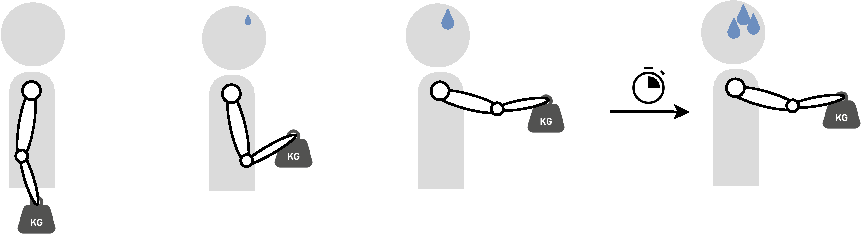
\includegraphics[width=\linewidth]{Chapters/imgs/baguette_carrying_fatigue.pdf}
    \caption{Illustration of the intuition about the changing nature of humans' physical abilities. When carrying a heavy object, putting it close to the body results in lower physical effort than if the object is further from the body. Moreover, even if the arm posture does not change, the effects such as muscular fatigue can cause that, over time, the level of necessary physical effort increases substantially. }
    \label{fig:baguette}
\end{figure}

% \todos{
% \begin{itemize}
%     \item the physical abilities of humans and robots to execute certain task evolve both in time and with their state 
%     \item for example if we carry an object, we all know that puttin it in front of our body with our arm streched is gonna be much harder than if our arm is close to our body
%     \item see \Cref{fig:baguette}
%     \item similar parallel can be made for robots
%     \item therefore in order to be able to help human optimally and use the full physical potential of robots we need to calcualte/estimate/measure their physical abilities in real-time
%     \item to guarantee safety and improve efficiency
% \end{itemize}
% }

Moreover, human's and robot's physical abilities are not constant, they vary with time and with their state, and can evolve significantly during the task execution.
This is something that we all know intuitively. For example, if we carry a heavy object in our hand, as illustrated on \Cref{fig:baguette}. We all know that having our arm close our body makes carrying much easier than if our arm is stretched in front of us. Additionally, even if our arm does not move, the effects of muscle fatigue can decrease our ability to carry the object and ultimately make us unable to do it after certain time.
Therefore, even though the weight of the object does not change, our capacity (physical ability) of carrying it can change significantly with the changing state (posture) of the arm, as well as different physiological factors such as muscular fatigue.
%These physical factors influence human's perceived effort while executing different tasks, condition their cognitive strategies for adapting their posture and in that way have a direct influence on the their safety and well-being.
Similar parallel can be made for robotic manipulators as well. 


Having an accurate online information about changing physical abilities of humans, enables assessing if the they are apt to execute a certain task and quantify if they need robot's assistance, due to their lacking physical abilities. On the other hand, accurate and online information about robot's changing physical abilities, enables creating robot control strategies that adapt to the their changes and exploit the robot's full physical potential. Therefore, to better assist humans and fully exploit robot's physical potential, tools capable of capturing their changing physical abilities in real-time are needed, adding an additional requirement
\begin{requirement}[{RQ\ref{req:online}}] \label{req:online}
     Enable capturing human's and robot's changing abilities online
\end{requirement}
% \begin{itemize}
%     \item \nameref{req:online}: Enable capturing human's and robot's changing abilities online
% \end{itemize}

% \todos{not very happy with the final two paragarphs.}
To go beyond qualitative characterisation of human-robot collaboration, the main focus of this thesis is therefore put on developing tools capable of capturing the changing physical abilities of humans and robots in real-time. In the long term this is anticipated as a necessary steps towards the enhancement of the collaboration and, overall, should contribute to the safety and well-being of humans at work.

As metrics characterising different physical abilities, for humans and robots, are numerous in the literature, \Cref{ch:inro_overview} brings an overview of commonly used ones and discusses their potential to address the requirements \nameref{req:task}-\nameref{req:online}.

% \todos{
% \begin{itemize}
%     \item physical ability metrics enable capturing such changes
%     \item therefore in order to be able to help human optimally and use the full physical potential of robots we need to calcualte/estimate/measure their physical abilities in real-time
%     \item the focus of this thesis is therfore put on developing tools capable of capturing their changing abilities in real-time and leveraging this information on the fly for enhancig the human-robot collaboratin scenarios
% \end{itemize}
% }

% \item therefore in order to be able to help human optimally and use the full physical potential of robots we need to calcualte/estimate/measure their physical abilities in real-time
% \item to guarantee safety and improve efficiency




%and polytopes enable capturing the changes in their abilities as well. Having an accurate information about the robot's physical abilities online, enables creating robot control strategies that adapt to the their changes and exploit the robot's full potential. On the other hand, having an accurate online information about the human's physical abilities is important for assessing if the operator is apt to execute a certain task and quantifying if the operator needs assistance of the robot due to its lacking physical abilities. Furthermore, having the real-time information about the operator's physical abilities enables ensuring that his abilities are never surpassed which has a direct impact on the operator's safety and well-being. Therefore, the collaborative workstations require creating more human-centred robot control strategies where the robot adapts its behaviour not just with respect to the requirements of the task and its own abilities, but also to the current abilities of the human operator as well as his safety. As polytope characterisations of robot's and human's physical abilities can be easily integrated with different robot control strategies, they have a great potential to be used for creating such adaptive collaboration scenarios.

\section{Characterising physical abilities}
\label{ch:inro_overview}
Many different metrics for characterising physical abilities of humans and robots are developed in the literature. They have a varying degree of complexity and physical interpretation, as well as different scope and accuracy.
Therefore, this section brings an overview of different physical ability metrics for robots and humans and discusses their potential use for human-robot collaboration.

\subsection{Metrics in robotics}
In robotics, physical abilities are characterised as different performance indicators, establishing the relationship between the robot's actuator limits (joint positions, velocities, torques, etc.), its kinematics and dynamics equations, and the achievable sets of different task related physical quantities, such as achievable positions, velocities, external wrenches and similar. The metrics quantifying different physical abilities are usually divided in two groups with respect to their scope: \textit{Global} and \textit{Local} metrics  \cite{russo2022measuring}. 

Global metrics present robot state independent metrics evaluated by taking in consideration all the possible robot states.
One example of such metric is the robot's reachable workspace \cite{Gosselin1991Synthesis,Vahrenkamp2016,kucuk2005robot}, characterising the set of \gls{cs} positions the robot can reach given its geometry and the limitations of its actuator's positions. More generally, workspace analysis based tools find the set of robot's reachable \gls{cs} positions given the limitations of its actuators, its kinematics and dynamics and different task related variables. Examples of such metrics are  constant orientation workspace \cite{Merlet1999Determination} representing robot's reachable positions with a given fixed orientation, singularity free workspace \cite{Jiang2008} representing the reachable positions without any singular configurations, or wrench closure workspace \cite{gouttefarde2006determination,Lau2011} which corresponds to robot's reachable positions guaranteeing the ability to apply certain set of wrenches.
One traditional application for such performance metrics is robot dimensional design, as they enable verifying and guaranteeing that the robotic system, being designed, is compliant with all the requirements of the tasks. 
However, these reachable workspace analysis tools have relatively complex geometry which can be challenging to exploit when it comes practical applications. 

A different set of global metrics, often specified in manufacturer's data-sheets, are different scalar metrics representing the robot's physical abilities based on finding the \textit{worst-case} (minimal) or \textit{best-case} (maximal) values of different task related values within the workspace. These metrics guarantee certain physical ability values for a given robot, such as robot's payload, its \textit{worst-case} carrying capacity, robot's \textit{worst-case} positioning accuracy or positioning repeatability \cite{russo2022measuring}. 
Therefore, they are often used to evaluate if a certain robotic system is suitable for a given task, and potentially compare between the robots from different manufacturers. However, such simplified metrics evaluating the robot's physical abilities, based on \textit{worst-case} scenarios, are in many cases largely underestimating robot's true capacity.

Furthermore, global metrics are computationally expensive as their evaluation requires sweeping through all the robot states, and they are typically calculated only once for a particular robot design or a given task. Moreover, as they are evaluated for entire set of robot's states, they are by design not capable of characterising the changing nature of the robot's physical abilities, that are state dependent (\nameref{req:online}).

Local metrics, on the other hand, are robot state dependant performance metrics which can be evaluated relatively efficiently for any given state. They characterise robot's task related physical abilities for a single robot state, as opposed to the global metrics which are calculated for all robot states. 
Additionally, as they enable quantitative comparison of the performance of different robot's states, they can be used as a base for different global metrics, in order to characterise robot's abilities in the whole workspace \cite{Zacharias2007}. The local metrics are often represented as scalar values indexes for a given robot's state \cite{Patel2015}, where some of the most well known ones are: manipulability index \cite{yoshikawa1985manipulability} and condition number \cite{Gosselin1991} which characterise the movement and dexterity capacity of the robot as well as its accuracy \cite{merlet_jacobian_2006}, dynamic manipulability \cite{yoshikawa1985dynamic} that characterises the task related acceleration capacity or the robot stiffness \cite{PASHKEVICH2011662} characterising the robot's tasks related load and deflection relationship.
Having a scalar metric is beneficial when it comes their use in different optimisation scenarios, for example in robot design refinement \cite{kucuk2005robot} or in robot trajectory generation \cite{Guilamo2006}. 


\begin{figure}
    \centering
    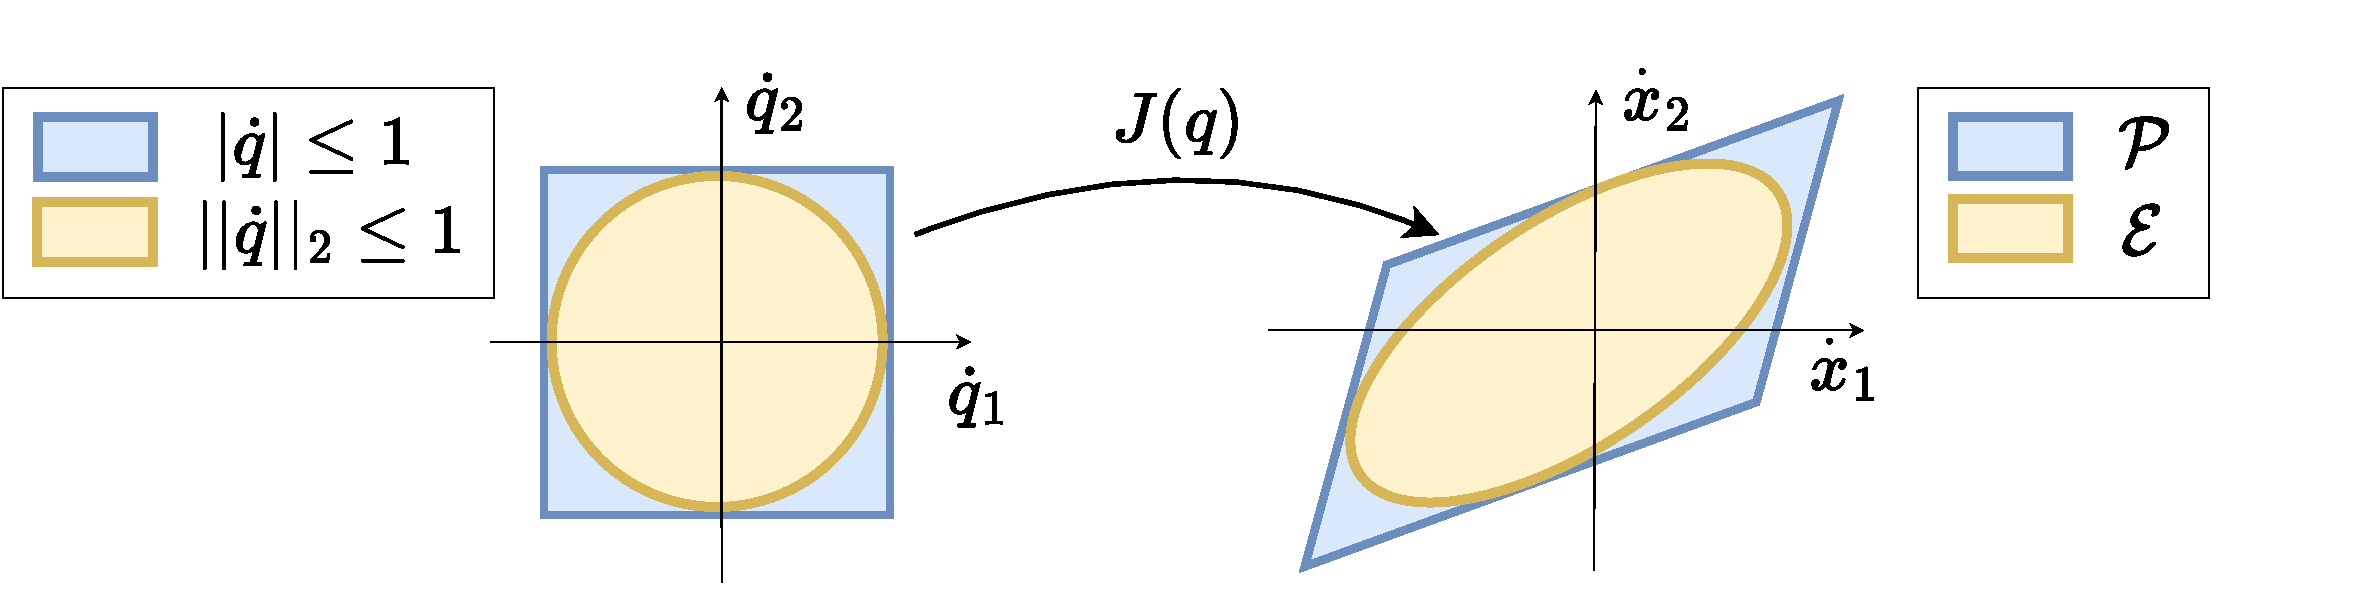
\includegraphics[width=0.8\textwidth]{Chapters/imgs/ellip_poly.pdf}
    \caption{An example manipulability polytope and ellipsoid geometry for a planar $m=2$ robot with $n=2$. The difference between the \gls{js} limits for ellipsoid described with $||\dot{\bm{q}}||_2\leq1$ (orange) and the range limits $\bm{-1}\leq\dot{\bm{q}}\leq\bm{1}$ (blue) is shown on the left. The difference in obtained achievable task space velocity $\dot{\bm{x}}$ polytope $\mathcal{P}$ (blue) and ellipsoid $\mathcal{E}$ (orange) is shown on the right plot. The plots show that both in joint and task space the ellipsoid metric is an underestimation of the true robot's capacity.}
    \label{fig:ellip_poly_dif}
\end{figure}


However having scalar representation of robot's capabilities can be constraining in certain applications, especially if the task has more than one dimension, for example movement in the 3D space. Different representations of robot's local physical abilities have been developed over the years that are capable of characterising the robot's task related capacity in the multi-dimensional task space. One particularly common representation is in ellipsoid form. Ellipsoids represent the ease of generating different task related variables (velocity, acceleration, inertia, stiffness etc.) in different directions of task space. One of the first ellipsoid shaped robot's physical ability representations was developed by \citet{yoshikawa1985manipulability} and is called the manipulability ellipsoid. Manipulability ellipsoid describes the capacity of a robotic system to generate task space velocities and can be described mathematically as
\begin{equation}
    \mathcal{E}(\bm{q}) = \left\{ \dot{\bm{x}} ~|~ \dot{\bm{x}} = J(\bm{q})\dot{\bm{q}},~~ ||\dot{\bm{q}}||_2 \leq 1 \right\}
\end{equation}
where $J(\bm{q})$ is robot's state $\bm{q}$ dependant Jacobian matrix relating its joint velocity $\dot{\bm{q}}$ and the task space velocity $\dot{\bm{x}}$\footnote{Task space velocity $\dot{\bm{x}}$ in general case can include both translational and rotational components, corresponding to the \gls{cs} twist. In that case $\dot{\bm{x}}$ is an abuse of notation, as there is no representation of a \gls{cs} pose $\bm{x} \in SE(3)$ which time derivative is a twist. Yet, for the sake of conciseness this notation is used throughout this manuscript.}. This metric evaluates the capacity of generating different task space velocities $\dot{\bm{x}}$ by considering that the robot can generate all the joint velocities $\dot{\bm{q}}$ with equal ease, represented by the condition $||\dot{\bm{q}}||_2 \leq 1$. Similar ellipsoid based representations can be used to characterise the force capacity of robotic systems \cite{chiacchio_global_1991}, acceleration capacity \cite{yoshikawa1985dynamic}, inertia \cite{Asada1984}, stiffness \cite{ajoudani2015role}, etc. 
%\todo{few applications, say they are efficient to calculate}

The hypothesis of equal capacity (ease of generating motion, forces, accelerations etc.) for all the robot's joints, in general case, does not reflect the true nature of robot actuation capacity. Robots have different actuators for different joints that can have substantially different characteristics. Therefore, in order to evaluate more accurate robot's task space capacity (motion, force, acceleration etc.) their true limits have to be taken in consideration. The ellipsoid metrics can be extended to considering non-uniform robot actuation limits, by introducing scaling
\begin{equation}
    ||W\dot{\bm{q}}||_2 \leq 1, \quad W=\text{diag}\left(\left[\dot{q}_{1,max} ,~\dot{q}_{2,max} , ~\ldots\right]\right)^{-1}
    \label{eq:scaled_norm}
\end{equation}    
where scaling matrix $W$ normalises the robot joint velocity capacity. However, they still make the assumption that the limits can be represented in the euclidean norm  $||.||_2$ form, implying that the robot's actuator limits are mutually interdependent, which in a general case is not true \cite{Lee1997manip}. Furthermore, as the real robot limits are usually expressed in a form of independent ranges $ \dot{\bm{q}}_{min} \leq \dot{\bm{q}} \leq \dot{\bm{q}}_{max}$, the euclidean norm (\ref{eq:scaled_norm}) based representation is an underestimation of the true robot's capacities. This effect is shown on the example of manipulability ellipsoid metric on \Cref{fig:ellip_poly_dif}. 

Once the true robotic actuator limits are considered, the representation of physical abilities becomes convex polytope shaped. As opposed to the manipulability ellipsoid $\mathcal{E}$, manipulability polytope can be defined as
\begin{equation}
    \mathcal{P}(\bm{q}) = \left\{ \dot{\bm{x}} ~|~ \dot{\bm{x}} = J(\bm{q})\dot{\bm{q}},~~ \dot{\bm{q}}_{min}\leq\dot{\bm{q}} \leq \dot{\bm{q}}_{max} \right\}
\end{equation}
The manipulability polytope $\mathcal{P}$ represents an exact solution of the robot's task space velocity capacity, given robot's state $\bm{q}$
and its joint velocity limits $\dot{\bm{q}}$. The difference between the manipulability ellipsoid $\mathcal{E}$ and polytope $\mathcal{P}$ is shown for a simple 2D example on \Cref{fig:ellip_poly_dif}.

Furthermore, as discussed by \citet{Finotello1998}, polytopes allow for calculating many other local performance metrics, such as Maximum Available Value (MAV) corresponding to the highest achievable magnitude of the task space variable (velocity, acceleration, force, static error, etc.), Maximal Isotropic Value (MIV) corresponding to the maximal value achievable in all the directions in space or Directional Index (DI) \cite{boschetti_minto_2023} corresponding to the maximum achievable task space variable in certain direction in space. Additionally, polytope volume and major (preferred) axis can be used as performance metrics as well \cite{chiacchio_global_1991, Long2018Evaluating}.

Therefore, polytope based physical ability metrics are the most complete local representation of task space physical abilities of robotic systems and they are used to characterise many task related physical values such as velocities \cite{Lee1997manip, long_constrained_2020}, forces \cite{chiacchio_evaluation_1996}, accelerations \cite{chiacchio_2000}, stiffness \cite{ajoudani2015role}, positioning accuracy \cite{pholsiri2005real}, etc.
The main downside to the polytope based metrics, with respect to the ellipsoid based metrics, is their computational complexity, making their use somewhat limited to non time critical applications.
% \todos{say that most of the stuff done with other metrics can be done with polytopes as well}

% \todos{
% \begin{itemize}
%     \item for robotics
%     \begin{itemize}
%         \item used to evaluate the robot capacity to execute certain tasks
%         \item to design more capable robots
%         \begin{itemize}
%             \item different visual metrics cable of being used to guarantee stuff
%             \item usually calculated in advance for the whole robot workspace 
%             \item payload for example, or reachable workspace, or wrench closure workspace for parallel robots
%             \item typically not taking in consideration robot's dynamics
%         \end{itemize}
%         \item to exploit robot's full potential when controlling it (or planning its movements)
%         \begin{itemize}
%             \item used in optimisation
%             \item different scalar metrics that are easy to calculate in real-time
%             \item manipulability index, and all the other indexes from the overview paper
%             \item also ellipsoids were used for this to find the directions with max movement capacity
%         \end{itemize}        
%     \end{itemize}        
% \end{itemize}
% }

\subsection{Metrics for humans}

Evaluating physical abilities of humans is a much more challenging than for robotic systems, as human bodies are much more complicated systems that depend both on biological and biomechanical, as well as cognitive and psychological factors.

Measuring different physical abilities of human subjects is traditionally done experimentally. The ability of human subjects to achieve different physical quantities such as generate forces \cite{HODDER2016Testing,HOLZBAUR20072442}, reach positions \cite{CASTRO2019108}, execute movements \cite{Jessop2016} or generate stiffnesses \cite{Tsuji1995,Artemiadis2010}, is tested in laboratory environment for a set of predefined human postures or movements. These experiments enable finding precise physical abilities of one or multiple subjects, for the tested motions and postures.  Such experimental analysis are common tools for evaluation of physical abilities in sports \cite{Jessop2016}, where the motions and postures of interest are usually well defined, and in rehabilitation \cite{HAISMA2006741} where the aim is to measure the progress of the human subject's recovery. However due to the large variability in human bodies and movements, it is challenging to generalise these results to the human subjects who were not part of the experiments, as well as to different postures and movements, of the same human subjects, that were not tested in the experiments.

In more varied and unstructured settings, where the human postures and movements are harder to characterise, such as in factory setting, the experimental metrics are impractical. For these scenarios, instead of characterising the physical ability of human subject directly, different metrics are developed aiming to evaluate the ergonomics of human postures and movements when executing tasks. These metrics are able to account for variations in human body anthropomorphic structure as well as for different movement and forces generation requirements of the tasks. Such metrics are often defined in a form of standards, such as \gls{reba} \cite{reba}, \gls{rula} \cite{rula} or DULA and DEBA \cite{Yazdani2022} (their differentiable equivalents), and manuals, such as Great Britain's \textit{Manual Handling Operation Regulations} \cite{health1992manual} or NASA's \textit{Man-systems integration standards} \cite{nasa}. These metrics are designed to give a certain score or a recommendation for the human postures, movements or force generation requirements of the task, in order to evaluate if the task is well suited for human's physical abilities. Common applications of these metrics, in factory settings, have for a goal to evaluate and improve the ergonomics of human's tasks \cite{Busch2017} and workplace layouts \cite{ORE20161, Lietaert2019}. However, these metrics, in order to be task and human subject agnostic, make coarse approximations of human physical abilities which are constraining when it comes to the online human-robot collaboration scenarios \cite{maurice2015}. 
%\todo{motivate better, a sentence about problems} 

In order to characterise human's physical abilities more finely, without the need for time consuming and impractical experimental evaluation, different metrics based on human musculoskeletal models are proposed. Human musculoskeletal models are relatively complete models of human bodies capable of describing different body's biological and biomechanical parameters as well as its rigid body dynamics. Musculoskeletal models are actuated by muscle-tendon units, capable of applying a range of contracting forces, accelerations and velocities. Similar to robotic systems, several global and local physical ability metrics, based on musculoskeletal models, can be calculated by evaluating how different limits of the muscles as actuators effect human's task related physical abilities, such as to generate forces or motions. 

Several global physical ability metrics based on musculoskeletal models are introduced in literature, such as human upper extremity reachable workspace \cite{Lenarcic1994,Kurillo2013} or comfortable reachable workspace \cite{Figueredo2021}, the comfortablility map of the reachable workspace of human's upper limbs evaluated using \gls{rula} and \gls{reba} ergonomics scores.  

In addition to the global metrics many robotics inspired local, state dependent, metrics have been developed as well. Different authors have used their ellipsoid based representations to asses the velocity (manipulability) \cite{Rezzoug2012manipulability}, force \cite{rezzoug_application_2012, lazinica_higher_2010}, acceleration \cite{khatib2009robotics} and stiffness \cite{Artemiadis2010} capacity of humans based on their musculoskeletal models. Several of these ellipsoids have been extend to the more complete polytope representation as well, such as force polytope \cite{lazinica_higher_2010, rezzoug_application_2012, carmichael_estimating_2013} and acceleration capacity polytope \cite{khatib2009robotics, demircan2012muscle}. As in the case of robotic systems, polytopes represent the exact solution to the physical ability evaluation for any given state of the musculoskeletal model. 

However, as the musculoskeleral models are only an approximation of the true physics of human bodies, the accuracy of calculated physical ability metrics relies entirely on the correspondence between the model and the human subject. Multiple experimental studies were conducted comparing the experimental data against the polytopes and ellipsoids obtained using musculoskeletal models, namely for the human upper limb force generation capacity \cite{biomechanics1010008, HERNANDEZ2015,lazinica_higher_2010}. Their results confirm that the polytopes correspond better to the experimentally obtained capacity of the human subjects. However, the results further underline the importance of having an appropriate musculoskeletal model of the human subject. Even though many strategies have been developed for fitting the musculoskeletal models to human subjects in the biomechanics literature mostly based on different forms of scaling \cite{Lund2015, Ziyun2019}, it is still an open field of research. 

With the assumption of an appropriate and well adapted human musculoskeletal model of the human subject, polytopes and ellipsoids present an accurate estimation of the human's task related physical abilities. 
Even though polytopes are more accurate estimation, ellipsoid based representations, due to their computational efficiency, are still a preferred choice when it comes to evaluating human's physical ability, especially in real-time applications. The difference in computational complexity between polytope and ellipsoid evaluation for musculoskeletal models is even more exaggerated than for the robotic systems. As the musculoskeletal models often have many muscles (often more than 50) final polytope geometry becomes complex which ultimately has a negative impact of their computation time.

% \todos{
% \begin{itemize}
%     \item for humans
%     \begin{itemize}
%         \item for humans the metrics are mush less exact, mostly empirical
%         \begin{itemize}
%             \item in labs
%             \item per subject
%             \item hard to generalize
%             \item takes time
%         \end{itemize}
%         \item simpler metrics 
%         \item used to evaluate the ergonomics of the human posture, his task or his workspace
%         \begin{itemize}
%             \item evaluated in-situ
%             \item different score based scalar metrics
%             \item ergonomics scores based on different metrics and manuals
%             \item rula, reba, payload manual, nasa and similar
%         \end{itemize}        
%         \item different set of metrics based on human miscalculate models
%         \item based on exact evaluation of different metrics (similar to robots)
%         \begin{itemize}
%             \item used to evaluate maximal human capacities
%             \item more or less all the metrics as for robots can be used
%             \item ellipsoids and polytopes to evaluate the maximal force capacity
%         \end{itemize}   
%         \item there are also those who try to combine the two
%         \item standards + musculoskeletal stuff
%         \begin{itemize}
%             \item comfortability metrics ( a combination of the two ) \cite{Figueredo2021}
%             \item however calculated in advance and relatively complicated to use, no dynamics
%         \end{itemize}   
%     \end{itemize}
    
% \end{itemize}
% }

\subsection{Physical abilities in human-robot collaboration}

Human's and robot's individual physical ability metrics have been used in different human-robot collaboration scenarios. Robot's physical abilities are often calculated in order to make sure that the task requirements comply with the robot's capacity. On the other hand, human's physical ability and ergonomics metrics are then used to design suitable robot behaviors in order to make the human's task and posture more ergonomic. Such collaboration strategies consider the robot to be an action vector with limited resources whose job is to improve the task performance and the human ergonomics at the same time. Examples of such human-centered collaborative scenarios are described by \citet{KIM2021102084}, where the robot adapts the position of the manipulated object in space in order to improve human's ergonomics, or in the context of exoskeleton control by \citet{carmichael2013admittance,carmichael_towards_2011} and \citet{petric2019assistive}, where the robot adapts to different assistance needs of the human operator.

However, when it comes to the collaboration scenarios where a human and a robot interact physically in order to execute a certain task, characterising their joint physical abilities is still an open research question. Human and robot physical abilities are often expressed in different ways, with different units and with fundamentally different metrics, making the procedure of combining them challenging. Therefore, in order to characterise their joint physical capacity, the first step is to express their individual physical abilities need in the same unified form. 

When it comes to multi-robot physical collaboration, \citet{chiacchio_global_1991} have shown that ellipsoid based metrics can be used to calculate their combined joint velocity (manipulability) capacity. The resulting joint capacity has an ellipsoid form as well.  However, in their formulation, the collaboration of multiple robots is essentially seen as one larger robot, combining all the joints of all the robots, resulting in the robot with $n=n_1 + n_2 + \ldots$ joints.
\begin{equation}
    \bm{q} = \begin{bmatrix}
        \bm{q}_1\\ \bm{q}_2 \\ \ldots
    \end{bmatrix}, \quad
    \dot{\bm{q}} = \begin{bmatrix}
        \dot{\bm{q}}_1\\\dot{\bm{q}}_2 \\ \ldots
    \end{bmatrix}, \quad
    J(\bm{q}) = \text{diag}([J_1(\bm{q}_1),~ J_2(\bm{q}_2),~\ldots])
\end{equation} 
Where $n_i$ is the number of joints, while $\bm{q}_i$ is the vector of joint positions and $J_i(\bm{q}_i)$ is the Jacobian matrix for each one of the robot's involved.

\begin{figure}[!h]
    \centering
    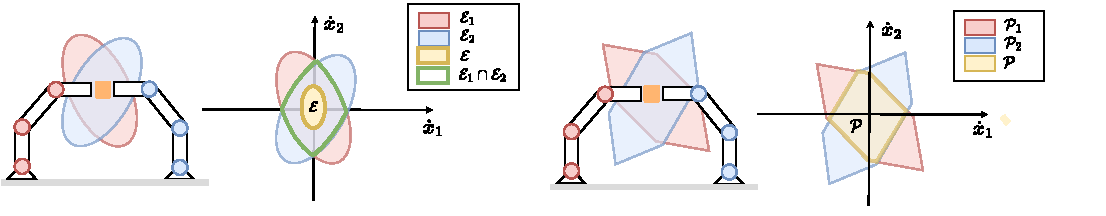
\includegraphics[width=1.05\linewidth]{Chapters/imgs/collab_manip_poly.pdf}
    \caption{Comparison of using ellipsoids (left) and polytopes (right) for collaborative physical ability calculation. Using polytopes, the common velocity capacity of the two robots is calculated as the intersection of their polytopes $\mathcal{P}=\mathcal{P}_1 \cap \mathcal{P}_2$. In ellipsoid case the intersection of the ellipsoids (green) is no longer an ellipsoid and it is hard to characterise, while the collaborative ellipsoid $\mathcal{E}$ (orange) introduced by \citet{chiacchio_global_1991} is a large underestimation of the true joint capacity.}
    \label{fig:collab_mani_poly}
\end{figure}
With such large number of joints, the euclidean norm $||.||_2$ limits present a large under-approximation of the real robot's limits, resulting in large under-approximation of the true capacity of the collaboration. As shown on the example on \Cref{fig:collab_mani_poly}, a more precise approach would be to intersect the ellipsoids calculated independently for all the robots $$\mathcal{E}=\mathcal{E}_1 \cap \mathcal{E}_2  \cap \ldots$$ However, the intersection operation over ellipsoids is hard to characterise and to evaluate, as the intersection of two ellipsoid is no longer an ellipsoid, and even if the intersection of the ellipsoids is obtained, it is just an approximation of true common capacity. 

Expressing the robot's physical ability in the polytope form however is not just the exact solution, but enables using the polytope algebra to do different operations, such as sum, intersection and Convex-Hull. These operations are well defined and can be calculated efficiently. The work from Jihong Lee \cite{lee2001velocity} shows that polytopes metrics can be used to describe the common velocity capacity of multi-arm collaborative robotic system.  The work describes an efficient way of calculating the joint velocity capacity by intersecting the individual polytopes of each one of the robots involved, resulting in a convex polytope shaped joint velocity capacity $$\mathcal{P}=\mathcal{P}_1 \cap \mathcal{P}_2  \cap \ldots$$
By exploiting different polytope algebra operations it is possible to express different physical collaboration scenarios as well. For example, if now the robots would be re-arranged from the parallel to the serial configuration, where the robot would be stacked one on top of the other, their joint velocity capacity would correspond to the Minkowski sum of their individual capacity $$\mathcal{P}=\mathcal{P}_1 \oplus \mathcal{P}_2  \oplus \ldots$$

\begin{figure}[!h]
    \centering
    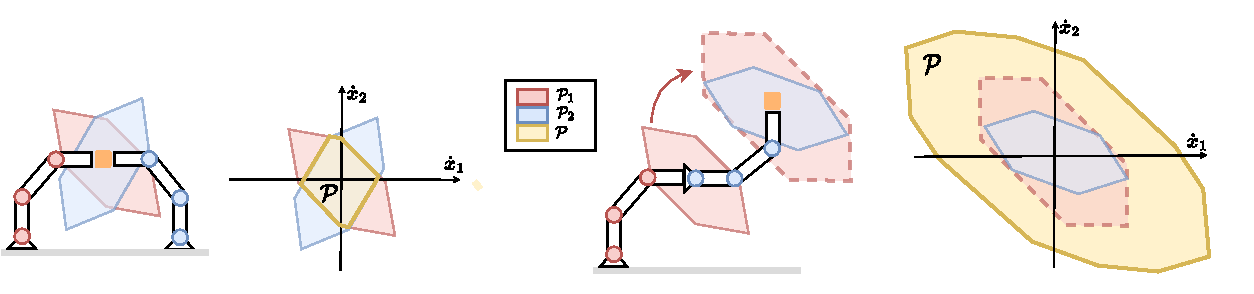
\includegraphics[width=\linewidth]{Chapters/imgs/collab_serial_parallel.pdf}
    \caption{Two examples of using polytope based metrics for joint achievable velocity capacity calculation of multiple robots collaborating. Figure on the left shows the parallel collaboration where the common capacity is calculated with the intersection. Figure on the right shows the serial collaboration where the common capacity is a Minkowski sum of their individual capacity. As the capacity is calculated at the end-effector of the second robot, the velocity polytope $\mathcal{P}_1$ of the first robot has to be transformed the same position (in red dashed border).}
    \label{fig:collab_serial_parallel}
\end{figure}
\Cref{fig:collab_serial_parallel} shows a simplified plannar example of the joint velocity capacity calculation for parallel and serial robot arrangement.

In summary, the polytope representation enables the physical abilities of robots, humans, and their collaboration to be expressed through a unified format. Furthermore, as many different physical abilities of humans and robots can be expressed in polytope form, it has the potential to provide an important set of tools for evaluating different collaboration tasks.
For example, by evaluating different physical abilities relevant to the task, it enables characterising if the task is more suitable for humans, robots or for different modes of their physical collaboration.  


% \todos{
% \begin{itemize}
%     \item what about collaboration metrics
%     \item Some metrics have been used but still very limited
%     \item when it comes to characterising their common capacity
%     \begin{itemize}
%         \item payload metrics might be used - very limiting
%         \item and ellipsoid based stuff from chiacchio - robots
%         \item lee also with polytopes a bit - robots
%         \item we still lack proper metrics to unify the humans and robots
%         \item they are usually expressed in different ways and hard to combine
%     \end{itemize}
%     \item Different ways of enhancing collaboration using physical ability metrics
%     \begin{itemize}
%         \item Collaborative workspace design for example - vincent paper
%         \item visualisation to the user 
%         \item Communicate the current robot state to the operator when collaborating
%         \item assist as needed control of exoskeletons also maybe (ellipsoids petric + polytopes carmichael)
%         \item but still not considering robot's capacity - robot only adapts to the human needs
%     \end{itemize}
% \end{itemize}
% }


\subsection{Why polytopes?}

As described in the previous sections, polytope representations of physical abilities accurately 
characterise the physical abilities of robotic manipulators, at the same time being the most accurate approximation of human physical abilities based on musculoskeletal models (\nameref{req:individual}). Additionally, since most of the well known polytope formulations for robotic systems can be formulated as polytopes for musculoskeletal models as well, they enable evaluating and comparing human's and robot's physical abilities in a unified manner. Furthermore, the polytope algebra enables operations over multiple polytopes and, in that way, has a potential to enable characterising common physical abilities of humans and robots involved in different physical collaboration scenarios (\nameref{req:common}).

Moreover, polytopes are local metrics, accurately representing different task related physical abilities for any robot's or human's state. Therefore, they enable capturing their state dependent changes in their physical abilities (\nameref{req:online}).

Polytopes enable comparing the operator's changing physical abilities with the physical abilities required by the task. Such real-time information has a potential to improve the operator's safety and well-being, by enabling to create assistive robot control strategies that adapt to the operator's changing capacity and make sure that they are never surpassed (\nameref{req:safety}). 
Similar human-centred and assistive robot control strategies are used in the context of assistive exoskeletons, as a part of so called \gls{aan} \cite{carmichael2013admittance} control paradigm. Using the \gls{aan} control strategy, the robot provides assistance to the operator adapted to the operator's current physical ability, providing the assistance only where the operator needs it. In their work \citet{carmichael_towards_2011} have proposed to quantify the need of assistance of the operator as the lacking physical ability to execute a certain task.

%However, \gls{aan} strategies are often based on different approximations of human's physical abilities, mostly due to the high computational complexity of polytopes. For example, \citet{carmichael_towards_2011} used a coarse sampling-based approximation of human's force capacity, \citet{Aldini2021RealTime} used a learning based approach using polynomial fitting, while \citet{petric2019assistive} approximated human's force capacity using ellipsoids.


When it comes to using polytopes in practical applications, there are two standard ways of representing them: as a set of vertices (vertex representation) or as a set of inequality constraints corresponding to their faces (half-plane representation) \cite{fukuda2004frequently}. Transforming a polytope into these standard representations enables using different efficient tools from computational geometry and polytope algebra in order to do operations over polytopes, for example find minimal distance between polytopes \cite{Ong1997gjk}, polytope volume \cite{Lawrence1991Volume} or calculate the Convex-Hulls \cite{Barber1996}, Minkowski sums \cite{BARKI2009525}, intersections and unions of multiple polytopes \cite{Tiwary2008}. Additionally, it opens doors for different simplification strategies of polytopes, by finding the inner and outer approximations of polytopes using spheres \cite{Botkin1994} or cubes \cite{BEMPORAD2004151}.

When characterising physical abilities, transforming the polytopes to the vertex representation enables using efficient triangulation algorithms from computational geometry. Most of the standard visualisation tools can visualise such triangulated meshes in very efficient manner, even in real-time. 
In the context of human-robot collaboration, an example application of polytope visualisation is proposed by \citet{Zolotas2021}, where the  robot's velocity polytopes are used to inform the operator about the robot's movement capacity during the teleportation task. A similar application was recently proposed by \citet{Weistroffer2022Using}, where the polytopes  of robot's force capacity were displayed to the operator designing the collaborative workspace with the aim to improve its safety and ergonomics. 

Polytopes can be expressed as a set of linear inequalities $A\bm{x}\leq\bm{b}$, that can be integrated into different optimisation problems in a form of linear inequality constraints. Most of the standard \gls{qp} \cite{boggs_tolle_1995} and \gls{lp} \cite{GOLDFARB198973} solvers support the inequality constraints in an efficient manner. In robotics, typical examples of applications often based on different optimisation strategies are robot control and trajectory planning. In the context of human-robot collaboration, being able to express both robot's and human's physical abilities in the polytope form, opens doors for creating more flexible robot control (or trajectory planning) strategies, which take in consideration both robot's and human's physical abilities.

Therefore, polytope representation provides an accurate representation of both humans' and robots' physical abilities in a unified manner (\nameref{req:individual}). Leveraging the efficient tools from polytope algebra, polytopes have a potential to enable characterising the common physical abilities of humans and robots interacting physically when executing certain task (\nameref{req:common}). Furthermore, being a local metric, polytopes enable capturing the changing physical abilities of humans and robots evolving with their state (\nameref{req:online}). Finally, by capturing human's changing physical abilities online, polytopes enable evaluating if the operator lacks the physical ability to execute certain task, and in that way evaluate his safety and well-being (\nameref{req:safety}). 

Furthermore, representing robot's and human's capacities in the polytope form enables using many efficient tools form the polytope algebra and computational geometry to perform operations over polytopes and to extract useful information concerning the task, for example different performance indicators. Additionally, polytopes can be transformed to more standard forms such as a set of vertices or set of inequalities which can then be used with standard visualisation tools and integrated in different optimisation problems, opening many doors in human-robot collaborative applications.

However, due to the considerable computational complexity of polytope evaluation, their applications in real-time (time-critical) applications is still relatively limited. 

\section{Thesis overview}

This thesis focuses on exploiting the polytope representation of human's and robot's physical abilities, as the most accurate characterisation of their abilities that is at the same time capable of fulfilling all the requirements \nameref{req:task}-\nameref{req:online}. 

The first two chapters (\Cref{ch:phisical_ability_metrics,ch:transformin_polytopes}) concentrate on the common formulations of the physical ability polytopes and their efficient evaluation.

In the effort to unify the vision of different physical abilities of humans are robots, \Cref{ch:phisical_ability_metrics} provides an overview of common polytope representations of their physical abilities. Furthermore, the chapter explores the combination of their individual polytopes in order to characterise their joint abilities as one single system.
Finally, the chapter proposes a synthesis of the common polytope formulations of humans and robots in a generic unified form.


% \todos{
% \begin{itemize}
%     \item \Cref{ch:phisical_ability_metrics} concentrates on polytopes and provides the overview of common polytope representations of physical abilities for humans robots and their collaboration as one single system
%     \item it proposes a synthesis (a unifying view) on the common polytope formulations
% \end{itemize}
% }

\Cref{ch:transformin_polytopes} focuses on transforming the introduced polytope formulations to their standard representations. The chapter introduces the generic families of polytope formulations derived from the unified generic formulation described in the previous chapter. The chapter then brings the overview of the standard polytope evaluation algorithms suitable for each one of the proposed families and discusses briefly their computation complexity. The chapter then introduces two new efficient algorithms (VEPOLI$^2$ and ICHM) developed in the context of this thesis, evaluates their computational efficiency and compares them to the state of the art methods. The experimental validation shows that the proposed algorithms have significantly lower computational complexity with respect to the standard approaches and have the potential to be used in online applications.  


% \todos{
% \begin{itemize}
%     \item \Cref{ch:transformin_polytopes} focuses on transformin the polytope formulations introduced in their standard representations, that can be used with practical applications
%     \item it fisrst introduces the generic families of polytope formulations present in physical ability polytopes
%     \item then it introduces an overview of the standard algorihtms suitable for these families and discusses briefly their comuptation complexity
%     \item then it introduces two new algorihtms develope in the context of this thesis and discusses their computational efficiny an provides their comparison with the state of the art methods. 
% \end{itemize}
% }

The following three chapters (\Cref{ch:physical_interaction,ch:informaiton_polytopes,ch:topca}) present applications of the real-time evaluation of human's and robot's physical abilities in a polytope form, with the aim to improve different aspects of the human-robot collaboration.


\Cref{ch:physical_interaction} presents the application of the real-time polytope evaluation for enhancing human-robot physical collaboration. The chapter aims to demonstrate that the real-time evaluation of the physical ability polytopes enables creating the robot control strategies capable of adapting to their changes on the fly. The proposed collaborative robot control strategies are experimentally validated on a task consisting in collaborative carrying of a heavy object, inspired by the LiChiE project. Two experiments are presented: dual robot collaborative carrying and human-robot collaborative carrying. In the dual robot collaborative carrying task, two Franka Emika Panda robots jointly carry 12kg object, largely above their rated capacity (6kg). The results show that by having real-time information about both robots' carrying capacities, the proposed collaborative control strategy adapted to their changes in real-time and successfully distributed the weight of the object during the whole duration of the experiment. In the human-robot collaborative carrying experiment, a human operator and a Franka robot carry 7kg object. The experiment showed that, having online information about their changing capacity enabled to employ the robot's and human's physical potential without compromising their safety. Furthermore, even though neither the robot nor the human would have been able to carry the entire object's weight on their own, by collaborating they were able to accomplish the task.


% \todos{
% \begin{itemize}
%     \item \Cref{ch:physical_interaction} presents the experimental validation of the proposed algorithm in the context of human-robot physical interaction
%     \item the collaborative carrying task is used, motivated by the LiChiE project (maybe)
%     \item two scenarios are shown, dual robot collaborative carrying and human-robot collaborative carrying
%     \item the algorithms are used to calculate the polytopes in real-time and create robot control strategies that adapt to the changing phsyical abilities of humans and robots in real-time
% \end{itemize}
% }


\Cref{ch:informaiton_polytopes} explores the idea of using polytope representations of robot's physical abilities as real-time visual feedback to operators. The chapter discusses the potential of such visualisation to provide the operator with real-time insight into the robot's current state and its current physical abilities. The chapter introduces a new polytope formulation developed particularly with the visualisation in mind: the approximation of the robot's reachable space within a time horizon. This polytope formulation represents the \gls{cs} the robot can reach in a certain horizon time, from its current position, while respecting all the robot's actuator limits, its kinematics and dynamics. 
By representing the reachable space of \gls{cs} positions, once visualised, this polytope's interpretation is more intuitive in comparison to the other common polytope formulation representing abstract physical quantities (forces, accelerations, velocities, etc.). 
Moreover, in the effort to evaluate the effectiveness of the real-time polytope visualisation to the operators, 
\Cref{ch:informaiton_polytopes} presents the preliminary work on the development of the testing setup based on the \gls{ar} tools. This setup presents the foundation for the future work on evaluating the information sharing potential of different polytope formulations and different visualisation modalities, in the context of the human-robot collaboration. 


% \todos{
% \begin{itemize}
%     \item \Cref{ch:informaiton_polytopes} discusses the application of polytopes as real-time visual feedback to operators
%     \item The chapter introduces a new polytope formulation developed particularly with the visualisation in mind, reachable space within a time horizon
%     \item the chapter also brings the preliminary work on the developement of the visualisation testing platform based on Augmented reality tools
%     \item with the long-term goal to validate the efficiency of polytopes in sharing information and thier different visualisation modalities
% \end{itemize}
% }

\Cref{ch:topca} introduces the application of robot's movement capacity polytopes in the \gls{cs} trajectory planning.
The chapter shows that real-time evaluation of polytopes enables adapting to the changes in the robot's movement capacity on the fly and in that way to exploit its full movement potential.
The chapter proposes a \gls{cs} trajectory planning strategy that evaluates robot's movement capacity in each step of the trajectory execution and recalculates the optimal trajectory using the updated values in real-time.
By re-planning the trajectory in real-time, the proposed method is able to react on environmental changes as well.
The method's efficiency is confirmed using an experimental benchmark comparison with the state of the art methods. 
Finally, a practical utility of the proposed method is demonstrated in the experiment of the human-robot collaborative waste sorting, where the proposed method is used to generate efficient and reactive robot's movement on the fly.

% \todos{
% \begin{itemize}
%     \item \Cref{ch:topca} introduces the application of robto's movement capacity polytopes in the Cartesain space trajecotry planning.
%     \item the chapter shows that real-time evaluation of polytopes enables adapting to the changes in the robot's movement capacity in on the fly and in that way exploit its full potential
%     \item the by replaining in real-time the trajectory is able to account for environmental changes and the cahnges in the task as well
%     \item the method efficiency is confirmed using the exeprimental benchmark comparison with the state of the art methods. 
%     \item also an applicative experiment is provided in the context of human-rovot collaborative waste sorting
% \end{itemize}
% }

\Cref{ch:software} presents the \codet{pycapacity} package, an efficient framework for calculating different physical ability metrics for both humans and robots, based on polytopes and ellipsoids.
The package implements several state of the art algorithms for polytope evaluation and manipulation, including VEPOLI$^2$ and ICHM developed in the context of this thesis, bringing many of them to the interactive online capable execution times.
The package is open-source, easy to install, and has relatively extensive documentation. Furthermore, the package is written in an user-friendly way with the aim to facilitate building applications and potentially bring these metrics to the wider community


% \todos{
% \begin{itemize}
%     \item \Cref{ch:software} presents the  \codet{pycapacity} package, an efficent framework for calculating different phsyical ability metrics for both humans and robots, based on polytopes and ellipsoids.
%     \item the package implements several state of the art algorihtms for polytope evaluation and manipulation, bringing menay of them to the interactive online application 
%     \item the package is open-source, is easy to install  and is written in an user-friendly way with the aim to facilitate building applications and potentially bring these metrics to the wider community
% \end{itemize}
% }

\Cref{ch:thesis_conclusion} brings the thesis conclusion and the discussion on the perspectives of the physical ability polytopes in human-robot collaboration.


{

\defbibnote{pubthesis}{This section lists the publications published during the thesis period and the corresponding sections in the manuscript.
}
% \nocite{skuric2021robot,skuric2021common,Skuric2022human,Skuric2022hfr,skuric2023dynamics,pycapacity}
\newrefcontext[labelprefix=A]
\printbibliography[keyword={phd}, title=List of publications, heading=subbibnumbered, prenote=pubthesis]

Parts of the work proposed in the articles \cite{skuric2021robot} and  \cite{skuric2021common}, discussing methods of calculating common physical abilities of human-robot collaborations, are included in \Cref{ch:collab_metrics} of \Cref{ch:phisical_ability_metrics}. Furthermore, articles \cite{skuric2021robot,Skuric2022human,skuric2023dynamics} introduce two novel polytope evaluation algorithms (VEPOLI$^2$ and ICHM), described in \Cref{ch:transformin_polytopes}, as well as their experimental validation in the context of human-robot physical interaction, described in \Cref{ch:physical_interaction}. 


The paper \cite{Skuric2022hfr} introduces a new polytope formulation intended for the interactive visualisation to the operator: the convex polytope of the robot's reachable space within a horizon. This work is included in \Cref{ch:hfr} of \Cref{ch:informaiton_polytopes}.


The open-source Python package \codet{pycapacity}, introduced in \cite{pycapacity}, is described in \Cref{ch:software} of the manuscript.


%TOPCA - \textit{in preparation for submission.}

}
% no relationship with thesis
{
\defbibnote{nopubthesis}{
These publications were published in the thesis period, but correspond to side research projects.
% \todos{I am not sure about this one, I will probably remove these papers.}
}
\nocite{Zhen2020RWM, Skuric2022simplefoc}
\newrefcontext[labelprefix=B]
\printbibliography[keyword={phd_out}, title=Other publications during the thesis, heading=subbibliography, prenote=nopubthesis]



}

% \section{Publications}
% {
% \renewcommand{\bibsection}{\paragraph*{\bibname}}
% \nociteA{*}
% \bibliographystyleA{IEEEtranN}
% \bibliographyA{my}
% }